\documentclass{beamer} % bemutatóhoz: \documentclass{beamer}
\usepackage{t1enc}
\usepackage[english]{babel}
\usepackage{ragged2e}
\let\raggedright=\RaggedRight
\usepackage[utf8]{inputenc}
\usepackage{amsmath}
\usepackage{amsfonts}
\usepackage{amssymb}
\usepackage{amsthm}
\usepackage{mathrsfs}
\usepackage{mathptm}
\usepackage{physics}
\usepackage[]{algorithm2e}
\usepackage{times}
\newtheorem{lem}{Lemma}[section]
\newtheorem{theo}[lem]{Theorem}
\newtheorem{defi}[lem]{Definition}
\newtheorem{megall}[lem]{Megállapodás}
\newtheorem{allitas}[lem]{Állítás}
\newtheorem{atfog}[lem]{Átfogalmazás}
\DeclareMathOperator{\dom}{dom}
\DeclareMathOperator{\ess}{ess}
\DeclareMathOperator{\ch}{ch}
\usetheme{Madrid}
\setbeamertemplate{footline}[frame number]
\setbeamertemplate{navigation symbols}{}
\addtobeamertemplate{navigation symbols}{}{%
    \usebeamerfont{footline}%
    \usebeamercolor[fg]{footline}%
    \hspace{1em}%
    \insertframenumber/\inserttotalframenumber
}
\setbeamertemplate{caption}[numbered]
\title{On the list coloring of $k$-band buffering cellular graphs}
\subtitle{Master Thesis Presentation}
\author{Benjámin Martin Seregi}
\institute{
      
\includegraphics[scale=0.2]{KTH_Logotyp_RGB_2013}%
      \\[\medskipamount]
      KTH Royal Institute of Technology
}
%\titlegraphic{\includegraphics[]{elte_cimer_szines}}
\date{2018}
\begin{document}
\frame{\titlepage}
\begin{frame}
\frametitle{Problem Statement}
\begin{itemize}
\item Wireless communication has become an essential part of life 
\begin{itemize}
\item E.g. IEEE 802.11 (WiFi)
\end{itemize}
\item Dense deployment with limited spectrum
\item WiFi operates with 13/14 channels (3 non-overlapping\---Figure \ref{fig:wifi-freq})
\begin{figure}
\centering
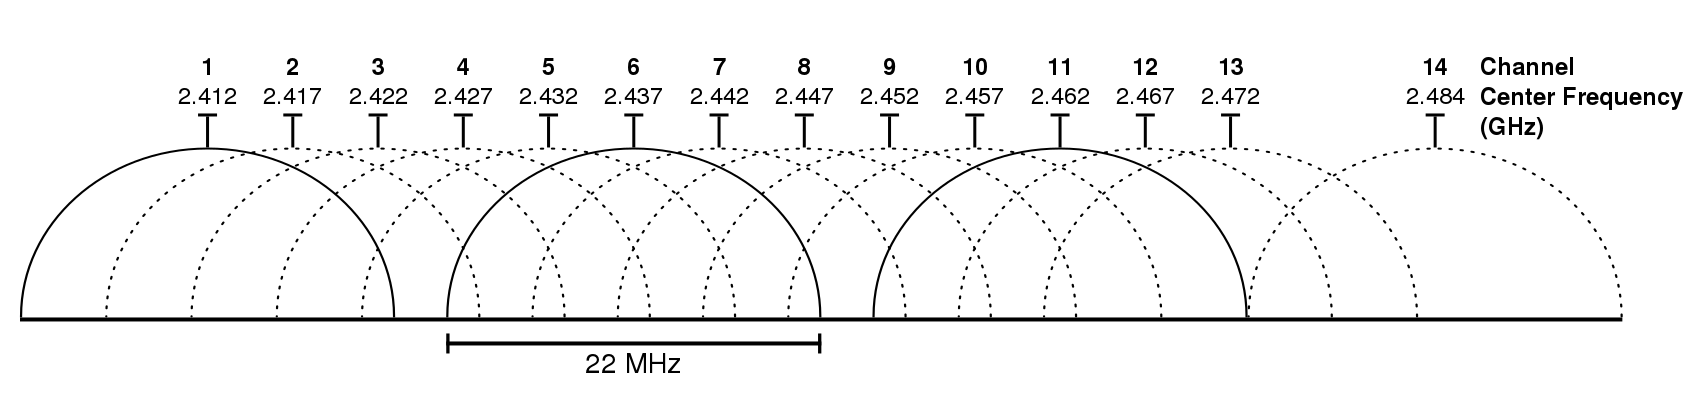
\includegraphics[scale=0.1]{figures/wifi-freq.png}
\caption{IEEE 802.11 channels By Liebeskind - Own work, CC BY 3.0, \url{https://commons.wikimedia.org/w/index.php?curid=14634575}}\label{fig:wifi-freq}
\end{figure}
\item Efficient utilization of the spectrum is extremely important
\begin{itemize}
\item Simultaneous transmission in overlapping channels $\leadsto$ interference
\item ''Neighboring'' access points (AP) should use different channels
\end{itemize}
\end{itemize}
\justifying
\end{frame}

\begin{frame}[allowframebreaks]
\frametitle{Background and Related Work}
\justifying
\begin{itemize}
\item Hexagonal tiling of the plane as a simplified model of wireless topologies
\end{itemize}
\begin{figure}
\centering
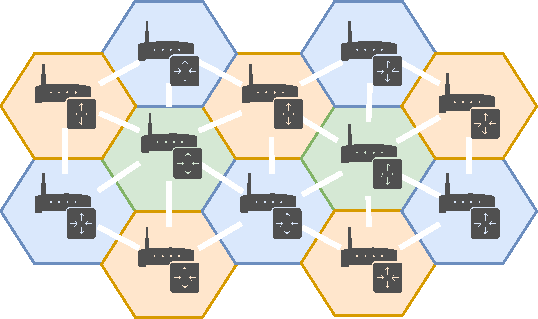
\includegraphics[scale=0.8]{figures/hexagonal-topology-wifi.pdf}
\caption{$1$-band buffering cellular graph colored with 3 colors}\label{fig:cellular-graph}
\end{figure}

\begin{defi}[$1$-band buffering cellular graph]  A graph $G$ is a $1$-band buffering \textit{cellular graph} (see Figure \ref{fig:cellular-graph}) if it is constructed from the hexagonal cell topology in the following way: each cell is a node and two nodes are connected if and only if they share a common boundary.
\end{defi}
\begin{defi}[$k$-band buffering cellular graph] Let $G$ be a $1$-band buffering graph cellular graph. Then the graph power $G^k$ is called $k$-band buffering cellular graph.
\end{defi}

\begin{figure}
\centering
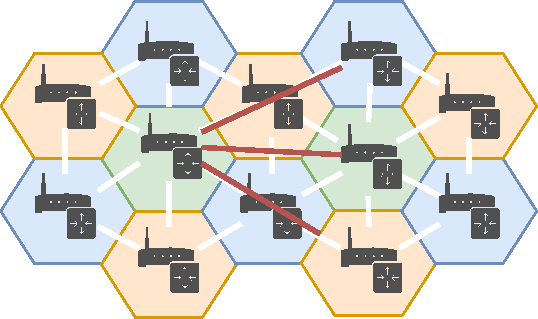
\includegraphics[scale=1]{figures/hexagonal-topology-wifi-2.pdf}
\caption{$2$-band buffering cellular graph with a non-admissible 3-coloring}\label{fig:cellular-graph-2}
\end{figure}


\begin{defi}
A channel allocation or coloring of a cellular graph is a function $c\colon V(G) \to F$ where $F$ is the available channels (colors) to the access points. A channel allocation (coloring) is called admissible (or proper) if and only if $(v_i,v_j) \in E(G)$ implies $c(v_i) \neq c(v_j)$ for all $i,j \in \lbrace 1, 2, \ldots, |V(G)| \rbrace$. An admissible coloring that minimizes $|c(V)|$ is called optimal, the number of color needed by an optimal coloring is the chromatic number of $G$ denoted by $\chi(G)$.
\end{defi}
\framebreak
\begin{itemize}
\item A. Sen et al. \cite{662943} calculated a lower and upper bound for distance-$k$ chromatic number of cellular graphs:
\end{itemize}

\begin{theo} The distance-$k$ chromatic number of a cellular graph $G$ is at least
\[ \begin{cases} 
      \frac{3}{4} \cdot (k+1)^2 & \text{if $k$ is odd} \\
      \frac{3}{4} \cdot (k+1)^2 + \frac{1}{4} & \text{if $k$ is even}.
   \end{cases}
\]
\end{theo}

\begin{theo} The distance-$k$ chromatic number of a cellular graph $G$ is at most $k^2 + k + 1.$
\end{theo}
\framebreak
\begin{itemize}
\item The set of free channels are constantly changing at each AP
\end{itemize}

\begin{figure}
\centering
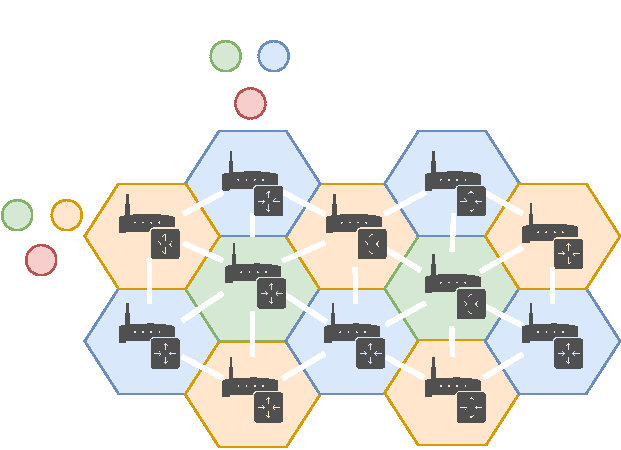
\includegraphics[scale=0.6]{figures/hexagonal-topology-wifi-list.pdf}
\caption{$2$-band buffering cellular graph with a proper 3-coloring from fixed lists}\label{fig:cellular-graph-list}
\end{figure}

\begin{defi} Let $G$ be a graph and $L(v)$ a set of colors for all $v \in V(G)$ such that $|L(v)|=k$ (see Figure \ref{fig:cellular-graph-list}). We say that $G$ is $k$\textit{-choosable} if $G$ is colorable such that the color of $v$ is in $L(v)$ for all $v \in V(G)$, such colorings called $k$\textit{-list coloring} of $G$.
\end{defi}
\begin{defi} The \textit{choice number} of $G$ is the smallest $k \in \mathbb{N}$ (denoted by $\ch(G)$) such that $G$ is $k$-choosable.
\end{defi}
\framebreak
\begin{itemize}
\item R. Wang et al. \cite{7248845} investigated the choice number of $2$-band buffering cellular graphs:
\end{itemize}
\begin{theorem}
Let $G$ be a $2$-band buffering cellular graph. Then $8 \leqslant \ch(G) \leqslant 10$.
\end{theorem}
\begin{itemize}
\item For $k > 2$, no upper bounds have been reported so far.
\end{itemize}
\end{frame}
\begin{frame}
\justifying
\frametitle{Research Methodology}
\begin{itemize}
\item Analytical approach to prove our upper bound
\item Computer simulation for validating the results
\end{itemize}
\end{frame}

\begin{frame}[allowframebreaks]
\frametitle{Results and Analysis}
\justifying
\begin{itemize}
\item A new bound has been established:
\end{itemize}
\begin{theorem} Let $G$ be a $k$-band buffering cellular graph. Then 
$$\ch(G) \leqslant \frac{3k(k+1)}{2} + 1.$$
\end{theorem}
\begin{itemize}
\item For $k=2$, we have $\ch(G) \leqslant 10$ which coincides the result of R. Wang et al. \cite{7248845}.
\item A polynomial algorithm has been developed that finds a proper list-coloring based on Galvin's theorem \cite{Galvin:1995:LCI:199352.199369}:
\end{itemize}

\begin{algorithm}[H]\label{alg:szekeres-list-coloring}
 \KwData{A $k$-band buffering cellular graph $G$ and a set of colors $L(v)$ for all $v \in V(G)$ with $|L(v)| \geqslant \frac{3k(k+1)}{2} + 1$}
 \KwResult{$\left(\frac{3k(k+1)}{2} + 1\right)$-list coloring of $G$}
  Let $G^*$ be the $k$-bounded acyclic orientation of $G$\;
  \While{$V(G^*)$ is non-empty} {
  	Let $\alpha$ be a color from $L(v)$ where $v \in V(G^*)$\;
  	$V_\alpha := \lbrace v \in V(G) \mid \alpha \in L(v) \rbrace$\;
  	Let $D$ be the subgraph of $G^*$ that $V_\alpha$ spans\;
  	Let $U$ be a kernel in $D$\;
  	Color the nodes in $U$ with color $\alpha$\;
  	Remove $\alpha$ from $L(v)$ for all $v \in V_\alpha$\;
  	Remove the colored nodes, that is, $V(G^*) := V(G^*) \setminus U$\;
  }
 \caption{$\left(\frac{3k(k+1)}{2} + 1\right)$-list coloring of a $k$-band buffering cellular graph}
\end{algorithm}
\end{frame}

\begin{frame}
\frametitle{Conclusions}
\justifying
\end{frame}

\begin{frame}
\justifying
\center
\textbf{Thank you for your attention!\\ Questions?}
\end{frame}

\begin{frame}[allowframebreaks]
        \frametitle{References}
        \bibliographystyle{amsalpha}
        \bibliography{references.bib}
\end{frame}
\end{document}